\chapter{Estado del Arte}
\label{chapter:Estado del Arte}


%%% SECTION
\section{Introducción}
El objetivo de este capítulo es realizar un análisis de los diferentes avances, desarrollos y tecnologías disponibles en el ámbito de la solución planteada. 

Este análisis tiene como objetivo identificar enfoques y metodologías en distintas áreas, como la extracción de información a partir de fuentes web, el análisis y procesado de texto y el uso de técnicas de Inteligencia Artificial aplicadas al Procesamiento de Lenguaje Natural.

De esta forma se puede establecer un contexto para el problema a resolver y justificar la elección de las tecnologías y metodologías a utilizar en el desarrollo de la solución propuesta.

\section{Problemática a resolver}

La búsqueda de ayudas y subvenciones es una tarea que la mayoría de las empresas, sobre todo las que tienen menos recursos, realizan en su día a día.
Para ello, existen diferentes plataformas de ayudas a empresas, algunas nacionales y otras de carácter internacional. 
Sin embargo, esta tarea puede resultar complicada y tediosa, ya que implica una búsqueda constante de nuevas posibilidades de financiacióna través de distintas fuentes.
Además, la información sobre estas convocatorias suele estar distribuidas en diferentes fuentes, desde las propias plataformas a documentación oficial del estado.
Esto supone que a la hora de realizar una búsqueda de posibles convocatorias de financiación, se acabe con un conjunto de fuentes con diferentes estructuras y formatos.

En la mayoría de los casos, las convocatorias suelen tener asociados diferentes documentos, en su mayoría en formato PDF, los cuales pueden ser extensos, y además usan un lenguaje técnico, típico de este tipo de documentos, que dificulta su comprensión.
Esto al final supone una complicación por parte de las empresas a la hora de acceder a información clave de las convocatorias de forma mas rápida, como requisitos, plazos, presupuesto o condiciones de participación.
Estos problemas de accesibilidad y estandarización de las convocatorias de ayudas suponen una barrera de acceso importante, que reduce las oportunidades de acceso a financiación para algunas empresas, y suponen una inversión en tiempo y esfuerzo en la tarea de búsqueda y filtrado por parte de éstas.

El desarrollo planteado en este proyecto pretende ser una solución a esta problemática, proporcionando una herramienta que sea capaz de identificar y extraer la documentación de las convocatorias, y aplicar técnicas de Inteligencia Artificial para extraer la información clave y dotarla de una estructura mas estandarizada, así como permitir la consulta de esta información de forma sencilla a partir de un agente conversacional.


\section{Soluciones disponibles}

Dejando a parte de momento las soluciones basadas en Inteligencia Artificial, las cuales se comentarán en secciones posteriores, existen diferentes metodologías para la búsqueda de información sobre estas convocatorias:

\subsection{Plataformas de convocatorias}

Existen diferentes plataformas que recopilan información sobre convocatorias de ayudas y subvenciones, a las cuales las empresas pueden acceder para explorar las diferentes opciones de convocatorias, y valorar si se ajustan a su situación.
Estos portales de convocatorias suelen estar disponibles en plataformas tanto gubernamentales como privadas, que recopilan y organizan la información sobre diferentes ayudas disponibles. 
Además, estas herramientas suelen permitir aplicar filtros en las búsquedas por diferentes características, como el área geográfica, el perfil de la empresa solicitante, o el tipo de ayuda.

\begin{itemize}

    \item \textbf{Portales de ayudas gubernamentales}:\\
    Las diferentes instituciones públicas suelen ofrecer portales informativos donde publican este tipo d econvocatorias, ya sean a nivel local, regional o nacional. Estos portales permiten visualizar estas voncovatorias, pero a un nivel básico en cuanto a experiencia de usuario, y aunque la totalidad de la información siempre está disponible, ya sea en el propio portal o mediante enlaces a diferentes fuentes documentales, el análisis y búsqueda de información clave es tediosa y lenta.    
    
    \begin{itemize}
        \item CDTI: Centro para el Desarrollo Tecnológico y la Innovación\cite{cdti}.
        \item Grupo SPRI\cite{spri}.
        \item SODERCAN: Sociedad para el desarrollo ragional de Cantabria\cite{sodercan}.
        \item Portal de ayudas del Ministerio para la Transofrmación Digital y de la Función Pública\cite{ayudasgob}.
        \item Andalucía Trade: Incentivos para Desarrollo Induatrial y Proyectos de I+D+i \\Empresarial\cite{atrade}.
    \end{itemize}

    \item \textbf{Plataformas privadas de información sobre subvenciones}:\\
    Algunas empresas recopilan información sobre ayudas a empresas, las estructuran en bases de datos y ofrecen el acceso a esta información como servicio, garantizando en éste la calidad de la información y una actualización constante del listado de ayudas disponibles.
    El inconveniente de estas plataformas es que, pese a ofrecer servicios de búsqueda que suelen tener interfaces mas amigables e información mas directa, suelen ser herramientas de pago, y el acceso completo a la información puede supoer un coste económico adicional.
    Algunos ejemplos de estas plataformas son Fandit \cite{fandit} u OpenGrants \cite{opengrants}.

\end{itemize}


\subsection{Web Scraping}

Una solución alternativa a la búsqueda manual en portales de ayudas es el uso de herramientas de Web Scraping.
El Web Scraping \cite{inbook} es una técnica utilizada para extraer información de sitios web de manera automatizada. Consiste en el uso de programas o scripts que navegan por páginas web, recopilan datos estructurados y los almacenan en un formato más accesible, como bases de datos o archivos locales JSON o CSV, por ejemplo. Esta práctica es ampliamente utilizada en diversos sectores para la recopilación y análisis de información a gran escala.

Generalmente el proceso de Web Scraping se desarrolla en varias etapas:

\begin{itemize}
    \item Solicitud HTTP: La herramienta de scraping envía una solitcitud HTTP a una página web para obtener su contenido.
    \item Extracción de datos: Se analiza el código fuente de la página, y según la configuración establecida en el scraper, se extraen los datos requeridos mediante comandos de parseo propios de la herramienta, expresiones regulares, o bots de navegación automatizada.
    \item Almacenamiento de la información: Una vez obtenidos los datos, estos se pueden formatear y almacenar según convenga en el caso de uso. 
\end{itemize}

Existen diferentes metodologías de Web Scraping:

\begin{itemize}
    \item \textbf{Análisis HTML}: En múltiples sitios web, se generan automáticamente grandes volúmenes de páginas a partir de fuentes de datos estructuradas, como bases de datos, mediante scripts o plantillas que organizan la información en formatos homogéneos. 
    En minería de datos, un wrapper es un programa que identifica plantillas en una fuente de datos, extrae su contenido y lo transforma en una estructura relacional. 
    La inducción de wrappers asume que las páginas de entrada siguen un patrón identificable, usualmente a través de formatos de URL comunes. 
    Además, lenguajes de consulta para datos semiestructurados, como XQuery y HTQL, permiten analizar, extraer y modificar información en sitios web HTML \cite{miningweb}.

    \item \textbf{Análisis DOM}: Los programas pueden acceder a contenido dinámico generado por scripts del lado del cliente mediante la integración de un navegador web, como Internet Explorer o Mozilla browser control \cite{domparsing}. 
    Estas aplicaciones analizan las páginas web y las estructuran en un árbol del Document Object Model (DOM), lo que permite extraer secciones específicas del contenido.
    El modelo DOM organiza una página web en una estructura arbórea, permitiendo su interpretación y almacenamiento a partir de una dirección web especificada, como ocurre en los motores de búsqueda. 
    Este enfoque ofrece gran flexibilidad y agilidad, ya que permite rastrear elementos presentes en la página sin depender de que el equipo de desarrollo web los exponga explícitamente en la capa de datos.

    \item \textbf{HTML DOM (Hyper Text Markup Language Document Object Model)}: Es un estándar para la obtención, manipulación y modificación de elementos HTML \cite{Gunawan}. 
    Define objetos y propiedades para cada componente HTML, así como métodos para acceder a ellos, optimizando la eficiencia del DOM.
    JavaScript, como lenguaje principal, permite acceder y manipular todos los elementos de un documento HTML a través del DOM. 
    En este modelo, cada elemento HTML se trata como un objeto, cuya interfaz de programación está compuesta por métodos y propiedades específicas.

    \item \textbf{Expresiones regulares (RegEx)}: Las expresiones regulares son fórmulas que definen patrones específicos para identificar conjuntos de caracteres en diversas cadenas de texto \cite{oreilywebacraping}. 
    Se componen de caracteres ordinarios y metacaracteres, los cuales modifican la interpretación del patrón.
    Aunque su sintaxis puede parecer compleja, las expresiones regulares son una herramienta esencial para el análisis y procesamiento de datos en cadenas de texto, por lo que es fundamental comprenderlas al menos a nivel básico.
    
    \item \textbf{XPath}: XPath es el componente principal del estándar XSLT (Stylesheet Language Transformation) y se utiliza para navegar y seleccionar elementos y atributos dentro de documentos XML \cite{asikri}. 
    Además, puede aplicarse en documentos HTML.
    XPath funciona como un lenguaje de selección de nodos en estructuras XML, siendo la expresión más utilizada la ruta de ubicación (location path). 
    Esta ruta emplea al menos un paso de ubicación para identificar un conjunto de nodos dentro de un documento. 
    La forma más simple es la selección del nodo raíz del documento, representada por el símbolo "/" , que también es el indicador del directorio raíz en sistemas de archivos Unix.
    
    \item \textbf{Reconocimiento de anotaciones semánticas}: Las páginas extraídas pueden incluir metadatos, marcas semánticas y anotaciones que permiten identificar datos específicos \cite{inbook}. 
    Por ejemplo, esta técnica puede considerarse un caso particular del análisis DOM si las anotaciones están integradas en las páginas, como ocurre con Microformat. 
    En otro caso, las anotaciones se almacenan y gestionan de manera independiente de las páginas web, organizándose en una capa semántica, de modo que los scrapers pueden obtener el esquema e instrucciones desde esta capa antes de realizar el raspado de las páginas.


\end{itemize}

En el ámbito del Web Scraping, específicamente con el lenguaje de Programación Python, podemos encontrar las siguientes librerías:

\begin{itemize}
    \item \textbf{BeautyfulSoup}: BeautifulSoup es una biblioteca de Python diseñada para el análisis, extracción y manipulación de datos en documentos HTML y XML. 
    Su funcionamiento se basa en la creación de un árbol de análisis sintáctico (parse tree), que estructura el contenido de la página web de manera jerárquica, permitiendo navegar por los nodos, buscar elementos específicos y modificar el contenido.
    BeautifulSoup admite múltiples analizadores (parsers), como lxml, html.parser y html5lib, cada uno con diferentes niveles de velocidad y compatibilidad. 
    Su sintaxis flexible permite localizar elementos a través de etiquetas, atributos y selectores CSS, facilitando la extracción de datos estructurados de páginas web. Además, cuenta con métodos para limpiar el contenido, eliminar etiquetas HTML y exportar la información en diversos formatos \cite{9274270}.

    \item \textbf{Scrapy}: Scrapy es un framework de Python diseñado para la extracción estructurada de datos mediante web scraping y crawling. 
    Su arquitectura modular permite gestionar solicitudes HTTP, procesar respuestas y almacenar datos de manera eficiente. 
    Scrapy opera a través de un flujo de trabajo basado en spiders, que son clases definidas por el usuario encargadas de especificar la lógica de extracción \cite{domparsing}.
    
    El motor de Scrapy (Scrapy Engine) coordina los componentes principales:
    
    \begin{itemize}
        \item Scheduler, que organiza las solicitudes pendientes.
        \item Downloader, que ejecuta las peticiones HTTP y recibe las respuestas.
        \item Spiders, que analizan y extraen información relevante.
        \item Item Pipeline, que transforma, valida y almacena los datos obtenidos en formatos como JSON, CSV o bases de datos SQL y NoSQL.
    \end{itemize}

    Además, Scrapy admite el uso de middlewares, tanto en el Downloader como en el Spider, para modificar solicitudes y respuestas, gestionar sesiones y evitar bloqueos mediante técnicas como rotación de proxies y user agents. 
    Su diseño asincrónico optimiza el rendimiento, permitiendo la extracción masiva de datos con alta eficiencia.

    \item \textbf{Selenium}: Selenium es un framework de automatización de navegadores de código abierto utilizado para la ejecución de pruebas y la extracción de datos mediante web scraping \cite{9142938}. 
    Su funcionamiento se basa en la interacción con páginas web a través de un WebDriver, que actúa como un controlador para manipular elementos de la interfaz de usuario, simular clics, completar formularios y desplazarse por el contenido dinámico generado mediante JavaScript.
    El ecosistema de Selenium está compuesto por varios módulos:

    \begin{itemize}
        \item Selenium WebDriver, que permite la automatización de navegadores como Chrome, Firefox y Edge mediante controladores específicos.
        \item Selenium Grid, que posibilita la ejecución distribuida de pruebas y scraping en múltiples máquinas.
        \item Selenium IDE, una extensión que facilita la grabación y reproducción de secuencias de prueba en navegadores.
    \end{itemize}

    Para realizar web scraping con Selenium, se inicia una sesión de navegador con el WebDriver, se navega a la URL objetivo, y se localizan los elementos deseados mediante selectores XPath o CSS. A diferencia de frameworks como Scrapy o BeautifulSoup, Selenium es ideal para interactuar con sitios que requieren ejecución de JavaScript o carga dinámica de contenido, aunque su rendimiento puede ser inferior debido a la sobrecarga computacional del manejo de un navegador real.

\end{itemize}

\subsection{Procesamiento de Lenguaje Natural}

El Procesamiento de Lenguaje Natural (NLP) es una disciplina de la inteligencia artificial y la lingüística computacional que permite a las máquinas interpretar, comprender, generar y manipular el lenguaje humano de manera estructurada \cite{nlpstate}. 
Su aplicación abarca desde la traducción automática y el análisis de sentimientos hasta la generación de texto y los asistentes virtuales.

El Procesamiento de Lenguaje Natural emplea diversas técnicas computacionales para la interpretación y manipulación del lenguaje humano. 
Estas técnicas pueden dividirse en métodos estadísticos, basados en reglas y de aprendizaje profundo, siendo ampliamente utilizadas en tareas como la clasificación de textos, el análisis de sentimientos y la traducción automática.

\begin{itemize}
    \item \textbf{Preprocesamiento de Texto}
        \begin{itemize}
            \item \textbf{Tokenización}: La tokenización es un proceso esencial en el Procesamiento de Lenguaje Natural que divide un texto en unidades denominadas tokens. 
            Existen varios tipos \cite{schmidt2024tokenizationcompression}, siendo los principales: tokenización por palabras, que separa el texto en palabras individuales y es efectiva en idiomas con delimitadores claros como el inglés; 
            tokenización por subpalabras, utilizada en modelos como BERT y GPT, que emplea técnicas como Byte Pair Encoding (BPE) para manejar vocabularios extensos y palabras fuera de vocabulario (OOV); 
            tokenización por oraciones, que segmenta el texto en unidades sintácticas más grandes basándose en puntuación y reglas lingüísticas; y tokenización por caracteres, útil en modelos de aprendizaje profundo y generación de texto. 
            La selección del método adecuado depende del idioma y la tarea específica, siendo crucial en aplicaciones como traducción automática, análisis de sentimientos y recuperación de información.
            
            \item \textbf{Lematización y Stemming}: Son técnicas empleadas para normalizar palabras reducciéndolas a su raíz morfológica \cite{steminglemmatization}. 
            El stemming elimina afijos mediante reglas predefinidas, sin considerar el contexto, lo que lo hace rápido pero propenso a errores (ejemplo: "running" → "run", pero "better" → "bet"). 
            En contraste, la lematización utiliza análisis morfológico y diccionarios lingüísticos para obtener la forma base correcta (ejemplo: "better" → "good"), ofreciendo mayor precisión. 
            Mientras que el stemming es más eficiente en grandes volúmenes de datos, la lematización es preferida en tareas como análisis de sentimientos, recuperación de información y traducción automática, donde la precisión semántica es crucial.
            
            \item \textbf{Eliminación de stopwords}: Las stopwords son palabras de alta frecuencia en un idioma que generalmente no aportan significado relevante en tareas de Procesamiento de Lenguaje Natural, como artículos, preposiciones y pronombres (ejemplo: "el", "de", "y", "pero"). 
            Se eliminan para reducir la dimensionalidad del texto y mejorar la eficiencia de los modelos de análisis de texto \cite{Sarica_2021}. 
            Bibliotecas como NLTK, SpaCy y Scikit-learn incluyen listas de stopwords predefinidas, aunque pueden personalizarse según la aplicación. 
            Si bien su eliminación es útil en tareas como búsqueda de información y clasificación de textos, en ciertos casos, como en análisis de sentimientos o generación de texto, pueden ser necesarias para preservar el contexto semántico.
        \end{itemize}

        \item \textbf{Análisis Morfosintáctico y Semántico}
        \begin{itemize}
            \item \textbf{Etiquetado gramatical (POS Tagging)}: Es una técnica del Procesamiento de Lenguaje Natural que asigna a cada palabra de un texto su categoría gramatical correspondiente (sustantivo, verbo, adjetivo, etc.) en función de su contexto \cite{postagging}. 
            Se basa en reglas lingüísticas, modelos estadísticos o redes neuronales para mejorar la precisión del análisis. 
            Herramientas como NLTK, SpaCy y Stanford NLP utilizan algoritmos como Hidden Markov Models (HMM) o Redes Neuronales Recurrentes (RNNs) para realizar esta tarea. 
            El POS Tagging es clave en aplicaciones como análisis de sentimientos, desambiguación semántica y traducción automática, ya que ayuda a comprender la estructura y significado del lenguaje.
            
            \item \textbf{Parsing sintáctico}: El parsing sintáctico o análisis sintáctico consiste en la construcción de la estructura jerárquica de una oración para comprender su sintaxis, identificando la relación jerárquica entre las palabras mediante árboles sintácticos o dependencias gramaticales \cite{zhang2020surveysyntacticsemanticparsingbased}. 
            Existen dos enfoques principales: el parsing basado en constituyentes, que descompone la oración en frases (sintagmas nominales, verbales, etc.), y el parsing basado en dependencias, que representa las relaciones entre palabras mediante un grafo dirigido. 
            Herramientas como NLTK, SpaCy y Stanford Parser emplean algoritmos como CYK, Earley o modelos de redes neuronales para esta tarea. 
            El parsing sintáctico es esencial en aplicaciones como traducción automática, generación de texto y comprensión del lenguaje natural, donde la estructura de la oración influye en su interpretación.
            
            \item \textbf{Reconocimiento de Entidades Nombradas (NER)}: Es una técnica que tiene como objetivo identificar y clasificar entidades dentro de un texto, como nombres de personas, lugares, organizaciones, fechas, entre otros \cite{roy2021recenttrendsnamedentity}. 
            Utiliza enfoques basados en reglas lingüísticas, modelos estadísticos o aprendizaje automático para detectar estas entidades en el contexto del texto. 
            Herramientas como SpaCy, NLTK y Stanford NER emplean modelos entrenados en grandes corpus de datos para reconocer entidades y asignarles una etiqueta adecuada. 
            El NER es crucial en aplicaciones como extracción de información, análisis de noticias, y búsqueda semántica, ya que facilita la identificación y categorización de información relevante dentro de grandes volúmenes de datos.
        \end{itemize}

        \item \textbf{Representación de Texto}
        \begin{itemize}
            \item \textbf{Bag of Words (BoW)}: Es una técnica de representación de texto que convierte éste en una matriz de características, donde cada documento se representa como un conjunto de palabras sin tener en cuenta el orden o la gramática \cite{bow}. 
            En el modelo BoW, cada palabra única en el corpus se convierte en una característica (o columna) y cada documento se representa como un vector en el que el valor de cada entrada corresponde a la frecuencia de la palabra en ese documento. 
            Aunque es simple y eficiente, BoW presenta varios inconvenientes, como la pérdida de contexto y el orden de las palabras, la alta dimensionalidad, la falta de captura de relaciones semánticas y la presencia de ruido en los datos, lo que puede afectar la precisión y la interpretación del modelo. 
            Esta técnica, sin embargo, sigue siendo útil en tareas como clasificación de texto, análisis de sentimientos y recuperación de información, pero sus limitaciones han llevado al desarrollo de enfoques más avanzados.
            
            \item \textbf{TF-IDF (Term Frequency - Inverse Document Frequency)}: Método que pondera términos relevantes dentro de un corpus \cite{tfidf}. 
            Es una técnica de representación de texto que asigna un peso a cada término de un documento, basándose en dos componentes: la frecuencia de término (TF), que mide cuántas veces aparece un término en un documento, y la frecuencia inversa de documento (IDF), que mide la importancia de un término dentro de un conjunto de documentos. 
            El cálculo de TF es sencillo y se basa en la cantidad de veces que un término aparece en un documento en comparación con el total de términos del documento, mientras que IDF ajusta el peso del término según su frecuencia en todos los documentos, penalizando las palabras comunes que aparecen en muchos documentos. 
            El resultado es un valor que refleja la relevancia de un término en un documento en particular dentro de un corpus. 
            TF-IDF es ampliamente utilizado en tareas como clasificación de texto, búsqueda de información y análisis de contenido, ya que ayuda a identificar términos significativos que son relevantes en el contexto de un conjunto de documentos. 
            Sin embargo, también presenta algunas limitaciones, como la incapacidad para capturar relaciones semánticas entre palabras y su dependencia de la estructura del corpus.
            
            \item \textbf{Word Embeddings}: Técnicas avanzadas de representación de palabras que convierte las palabras en vectores numéricos de alta dimensión \cite{almeida2023wordembeddingssurvey}. 
            A diferencia de las representaciones tradicionales como Bag of Words o TF-IDF, que tratan las palabras de manera independiente, los word embeddings capturan las relaciones semánticas y contextuales entre palabras, representando palabras similares en espacios vectoriales cercanos. 
            Modelos como Word2Vec, GloVe, FastText o los posteriores modelos de Embeddings asociados a Grandes Modelos del Lenguaje aprenden estas representaciones mediante redes neuronales entrenadas sobre grandes corpus de texto, aprovechando el contexto de las palabras en las oraciones para generar sus vectores. 
            Los word embeddings permiten capturar propiedades lingüísticas, como sinónimos, analogías y jerarquías semánticas, mejorando el rendimiento en tareas como traducción automática, análisis de sentimientos, clasificación de texto y respuestas automáticas. 
            Aunque potentes, los embeddings también presentan desafíos, como la dificultad para representar términos poco frecuentes o palabras con múltiples significados (polisemia).
        
        \end{itemize}

        \item \textbf{Modelos de Aprendizaje Automático y Profundo}
        \begin{itemize}
            \item \textbf{Modelos basados en aprendizaje automático clásico}: Utilización de algoritmos tanto supervisados como no supervisados, como regresiones logísticas, árboles de decisión, SVM, k-means o Random Forest, entre otros, para tareas de clasificación o clusterización de texto \cite{nlpml}.
            Estos modelos estan diseñados para trabajar con datos numéricos, por lo que es necesario aplicar técnicas de representación numérica de texto como las ya anteriormente comentadas.
            
            \item \textbf{Redes Neuronales Recurrentes (RNN) y LSTM}: Modelos diseñados para procesar secuencias de texto y capturar dependencias contextuales.
            Son arquitecturas de Deep Learning diseñadas para procesar datos secuenciales, lo que las hace especialmente útiles en Procesamiento de Lenguaje Natural. 
            A diferencia de los modelos tradicionales de Machine Learning, las RNN pueden capturar dependencias temporales en el texto, ya que su estructura permite que la información de estados previos influya en la interpretación de los siguientes \cite{schmidt2019recurrentneuralnetworksrnns}. 
            Sin embargo, las RNN convencionales presentan problemas con secuencias largas debido a la desaparición o explosión del gradiente. 
            Para solucionar esto, surgieron las LSTM, que incorporan puertas de memoria que regulan el flujo de información, permitiendo recordar dependencias a largo plazo de manera más eficiente \cite{staudemeyer2019understandinglstmtutorial}. 
            Estas redes han sido ampliamente utilizadas en tareas como traducción automática, generación de texto, análisis de sentimientos y reconocimiento de voz. 
            Aunque las LSTM han mejorado el manejo de secuencias largas, han sido en gran parte reemplazadas por arquitecturas más avanzadas como Transformers, que manejan contexto de manera más eficiente mediante mecanismos de atención.
            
            \item \textbf{Arquitecturas de Deep Learning basadas en Transformers}: Estas nuevas arquitecturas revolucionaron el Procesamiento de Lenguaje Natural al superar las limitaciones de las arquitecturas de Redes Neuronales anteriores, gracias a su capacidad para procesar secuencias en paralelo y capturar relaciones a largo plazo mediante el mecanismo de atención. 
            Introducidos en el paper "Attention Is All You Need" \cite{vaswani2023attentionneed}, los Transformers utilizan mecanismos de self-attention para asignar pesos a cada palabra en función de su relevancia dentro del contexto, lo que permite una comprensión más profunda del significado del texto. 
            Modelos como BERT (Bidirectional Encoder Representations from Transformers \cite{devlin2019bertpretrainingdeepbidirectional}), GPT (Generative Pre-trained Transformer \cite{yenduri2023generativepretrainedtransformercomprehensive}) y T5 (Text-to-Text Transfer Transformer \cite{raffel2023exploringlimitstransferlearning}) lograron en su momento avances significativos en tareas como traducción automática, generación de texto, análisis de sentimientos y respuesta a preguntas. 
            Estas arquitecturas destacan por su capacidad de preentrenamiento en grandes corpus de datos y posterior ajuste fino en tareas específicas, lo que ha permitido obtener resultados de vanguardia en múltiples aplicaciones de PLN. 
            Tomando como base estas arquitecturas, han aparecido en los últimos años los Grandes Modelos del Lenguaje (LLMs), dando origen al desarrollo de la llamada Inteligencia Artificial Generativa.
        \end{itemize}

\end{itemize}

Estas técnicas han permitido avances en aplicaciones como asistentes virtuales, generación de texto automatizada y motores de búsqueda, optimizando la interacción entre humanos y sistemas computacionales.






\section{Inteligencia Artificial Generativa}

La inteligencia artificial generativa (IA generativa) es un campo de la inteligencia artificial que se centra en la creación de contenido nuevo y original a partir de datos existentes. 
A través del uso de modelos de aprendizaje profundo y técnicas avanzadas de procesamiento de datos, la IA generativa es capaz de generar texto, imágenes, audio, video y otros tipos de contenido de manera autónoma y coherente.  
El desarrollo de la IA generativa ha sido impulsado por la evolución de arquitecturas de redes neuronales como las redes generativas adversarias (GANs) \cite{goodfellow2014generativeadversarialnetworks}, los modelos basados en transformers \cite{vaswani2023attentionneed} y los modelos de difusión \cite{yang2024diffusionmodelscomprehensivesurvey}. 
Estas tecnologías han permitido la generación de contenido con una calidad cada vez mayor, logrando resultados que pueden ser indistinguibles de los creados por humanos.  

Su impacto ha sido significativo en múltiples sectores. 
En la industria creativa, ha transformado el diseño gráfico, la producción audiovisual y la generación de música, facilitando la automatización de tareas y ampliando las posibilidades de expresión artística \cite{iagengraphicdesign}. 
En el ámbito de la ciencia y la tecnología, se ha utilizado para la síntesis de datos, el descubrimiento de fármacos y la optimización de algoritmos \cite{ding2024risegenerativeartificialintelligence}. 
En el sector empresarial, la IA generativa ha revolucionado el marketing, la generación de contenido automatizado y la personalización de experiencias para los usuarios \cite{genaibusiness}.  

A medida que la tecnología continúa evolucionando, la IA generativa se enfrenta a desafíos éticos y regulatorios \cite{Hagendorff_2024}, incluyendo cuestiones sobre derechos de autor, desinformación y uso responsable. Sin embargo, su potencial sigue expandiéndose, con nuevos avances que permiten aplicaciones aún más sofisticadas y accesibles para diversos campos.


Los modelos de IA Generativa emplean diferentes técnicas de aprendizaje profundo para generar contenido, optimizando la calidad, coherencia y realismo de los resultados.
Las arquitecturas de redes neuronales basadas en transformers, introducidos en el artículo "Attention Is All You Need" (Vaswani et al., 2017) \cite{vaswani2023attentionneed} son la base de muchos de los modelos de IA generativa actuales, incluyendo los modelos de la familia GPT, Gemini de Google y Claude de Anthropic. 
Su principal ventaja radica en su capacidad para procesar y generar texto, imágenes, código y otros tipos de datos de manera eficiente y con una gran coherencia contextual.

Los transformers emplean un mecanismo llamado self-attention, que les permite asignar pesos a diferentes partes de la secuencia de entrada para comprender mejor las relaciones entre palabras o elementos. el flujo de esta arquitectura funciona de la siguiente manera:

\begin{figure}[h]
	\centering
	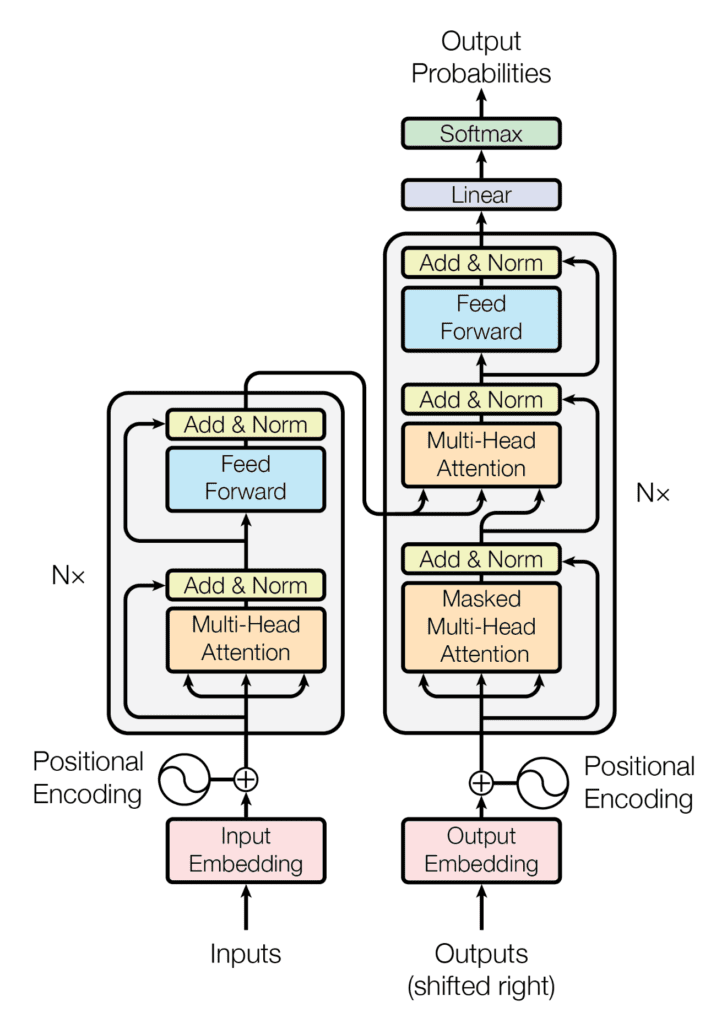
\includegraphics[width=0.6\textwidth]{figs/transformer_arquitecture.png}
	\caption{Arquitectura transformer}
	\label{fig:context-anoni1}
\end{figure}


\begin{itemize}
    \item \textbf{Codificación de entrada (Embedding Layer)}: Convierte los datos de entrada (por ejemplo, texto o imágenes) en vectores numéricos que representan cada elemento en un espacio multidimensional. En el caso del texto, se utiliza un embedding de palabras, que transforma cada token en un vector denso de alta dimensión.
    \item \textbf{Mecanismo de Self-Attention}: Permite que el modelo asigne importancia a diferentes palabras dentro de una oración o documento. Se basa en tres matrices: Query (Q), Key (K) y Value (V), que permiten calcular la relevancia de cada palabra con respecto a las demás. Se utiliza una función de Softmax para asignar pesos a cada conexión, ajustando la atención que se le da a diferentes partes del contexto.
    \item \textbf{Capas de Normalización y Feed-Forward}: Cada capa de atención es seguida por una red neuronal completamente conectada (feed-forward network) y una normalización de los datos para mejorar la estabilidad del entrenamiento.
    \item \textbf{Mecanismo de Positional Encoding}: Dado que los transformers no tienen memoria secuencial como las redes recurrentes, utilizan codificaciones posicionales para mantener el orden de los elementos en la secuencia. Estas codificaciones se agregan a los embeddings de entrada y permiten que el modelo distinga la estructura del texto.
    \item \textbf{Capa de Decodificación (para modelos generativos)}: En los modelos generativos, la salida del transformer se pasa a una capa de decodificación que genera una secuencia de salida basada en los tokens previos. Utiliza un enfoque autoregresivo, donde se genera un token a la vez y se retroalimenta al modelo para predecir el siguiente.
\end{itemize}

La inteligencia artificial generativa abarca diversas aplicaciones, como la creación de imágenes, texto, audio, video y modelos 3D. 
Sin embargo, debido a la naturaleza de este proyecto, nos centraremos principalmente en los grandes modelos de lenguaje, que son capaces de generar texto coherente y contextual a partir de indicaciones, transformando la interacción con la tecnología y facilitando la creación de contenido escrito de manera automática.

\section{Grandes Modelos del Lenguaje}

Los Grandes Modelos del Lenguage (LLMs) han generado gran atención debido a su sólido rendimiento en una amplia gama de tareas de lenguaje natural desde el lanzamiento de ChatGPT en noviembre de 2022. 
La capacidad de comprensión y generación de lenguaje de propósito general de los LLMs se adquiere mediante el entrenamiento de miles de millones de parámetros del modelo con grandes volúmenes de datos textuales. 
Aunque el área de investigación de los LLMs es muy reciente, está evolucionando rápidamente.

\subsection{Primeros modelos del lenguaje}

Con el auge de los Transformers, empezaron a surgir nuevos modelos cada vez mas complejos, incluyendo cada vez un volumen de parámetros mayor.
BERT (2018) marcó un punto de inflexión al introducir un preentrenamiento bidireccional basado en masked language modeling (MLM), mejorando la comprensión contextual en diversas tareas. 
Posteriormente, GPT-2 (2019) se centró en la generación de texto autoregresiva, destacando por su coherencia y fluidez, aunque con preocupaciones sobre su posible uso indebido. 
En paralelo, T5 (2019) propuso un enfoque texto a texto, permitiendo abordar múltiples tareas con una arquitectura unificada. 
La llegada de GPT-3 (2020) con 175B parámetros supuso un avance significativo en few-shot learning, posibilitando la generación de contenido sin necesidad de ajuste fino específico. 
Finalmente, LaMDA (2021) optimizó la interacción en diálogos abiertos, mejorando la coherencia en conversaciones de largo alcance y consolidando los avances en modelos conversacionales. 

\subsection{ChatGPT (2022)}
El lanzamiento de ChatGPT por OpenAI en noviembre de 2022 marcó un hito significativo en la evolución de los modelos de lenguaje, especialmente en aplicaciones de interacción conversacional. 
ChatGPT es una versión mejorada de GPT-3, que fue afinada específicamente para mejorar la calidad de los diálogos y la coherencia en respuestas a preguntas abiertas y conversaciones continuas. 
ChatGPT se entrenó utilizando un enfoque de Reinforcement Learning from Human Feedback (RLHF), donde los humanos proporcionaron retroalimentación activa sobre las respuestas generadas, lo que permitió al modelo mejorar su capacidad de ofrecer respuestas más relevantes, precisas y menos propensas a producir información errónea o sesgada.



\subsection{GPT-4 (marzo 2023)}

En marzo de 2023, OpenAI lanzó GPT-4, un modelo significativamente más avanzado que GPT-3 y ChatGPT. 
Con una capacidad de procesar entradas multimodales (texto e imágenes), GPT-4 permitió nuevas aplicaciones en áreas como análisis de contenido visual y descripciones detalladas. 
Además, mostró mejoras significativas en razonamiento complejo, en la resolución de problemas matemáticos avanzados y en la comprensión de contextos más largos.

sus principales características son:

\begin{itemize}
    \item Multimodalidad: GPT-4 podía procesar imágenes junto con texto, lo que le permitió realizar tareas como la interpretación de gráficos, la descripción de imágenes y la creación de contenido visual a partir de texto.
    \item Razonamiento mejorado: El modelo mostró un mejor desempeño en tareas que requieren razonamiento lógico y la capacidad de resolver problemas complejos.
    \item Mayor capacidad de manejo de contexto: A diferencia de GPT-3, GPT-4 pudo gestionar contextos más largos, lo que resultó en una mayor coherencia durante conversaciones extensas.    
\end{itemize}

% meter Incorporación de GPT-4 en Productos Comerciales (2023)
% Tras el lanzamiento de GPT-4, OpenAI lo integró en varios productos comerciales, como Microsoft Copilot (en herramientas como Word, Excel y otras aplicaciones de Microsoft 365) y Azure OpenAI Service. Estas integraciones proporcionaron una interfaz sencilla para que las empresas y los desarrolladores pudieran utilizar la potencia de GPT-4 para generar contenido, automatizar tareas y mejorar la productividad en diversas industrias.

% Aplicaciones clave:

% Automatización de procesos empresariales: GPT-4 se utilizó para mejorar la productividad en la automatización de procesos empresariales, como la generación de reportes, análisis de datos y respuestas automáticas.

% Generación de contenido: Integración en plataformas de generación de contenido para redactar artículos, correos electrónicos y otros textos comerciales.

% Asistentes virtuales avanzados: Mejora significativa en la creación de asistentes virtuales más inteligentes y capaces de manejar tareas complejas de atención al cliente.

\subsection{LLaMA (febrero 2023)}

LLaMA (Large Language Model Meta AI), lanzado por Meta (anteriormente Facebook) en 2023, se presentó como un competidor directo de GPT-3 y GPT-4. 
LLaMA se desarrolló con un enfoque en ser un modelo de gran escala, pero de mayor accesibilidad para la investigación académica y la comunidad de código abierto. 
LLaMA está diseñado para ser más eficiente y eficaz, permitiendo a los investigadores utilizar modelos de lenguaje a gran escala sin la necesidad de grandes cantidades de infraestructura.

Características clave de LLaMA:
\begin{itemize}
    \item \textbf{Accesibilidad}: Meta liberó versiones de LLaMA con diferentes tamaños de parámetros, haciendo posible que se usaran en equipos de investigación más pequeños.
    \item \textbf{Desempeño a gran escala}: A pesar de que LLaMA no es tan grande como GPT-4, mostró un rendimiento comparable en tareas de procesamiento de lenguaje natural (PLN).
    \item \textbf{Eficiencia}: El modelo fue diseñado para ser más eficiente en términos de uso de recursos, lo que lo hacía más accesible para investigadores en lugar de depender de poderosas infraestructuras.
\end{itemize}

LLaMA ayudó a democratizar el acceso a modelos de lenguaje de gran escala, permitiendo que más organizaciones y académicos participaran en la investigación y desarrollo de modelos avanzados.

\subsection{DeepSeek (junio 2023)}
DeepSeek es un modelo propuesto por DeepMind en 2023, cuyo enfoque se centra en la búsqueda semántica profunda y la comprensión avanzada de consultas complejas. 
Este modelo es particularmente útil en sistemas de búsqueda y recuperación de información, donde se requiere un entendimiento más allá de las coincidencias exactas de palabras clave, permitiendo la interpretación semántica de las consultas.

Características principales de DeepSeek:
\begin{itemize}
    \item \textbf{Búsqueda semántica avanzada}: DeepSeek está optimizado para interpretar y responder a consultas complejas, mejorando la precisión de las búsquedas más allá de simples coincidencias de términos.
    \item \textbf{Comprensión del contexto}: Utiliza técnicas de procesamiento de lenguaje natural para interpretar el significado detrás de las consultas, lo que permite ofrecer resultados más relevantes y contextualizados.
    \item \textbf{Aplicaciones en la búsqueda web y bases de datos}: DeepSeek ha demostrado ser particularmente útil en la mejora de los motores de búsqueda, brindando una mejor experiencia al usuario mediante la entrega de resultados más precisos y personalizados.
\end{itemize}

DeepSeek es un ejemplo del progreso continuo hacia el entendimiento más profundo del lenguaje y su aplicación en la búsqueda semántica, un área clave en la IA.


\subsection{LLaMA 2(julio 2024) AMPLIAR}

Meta lanzó LLaMA 2, mejorando la eficiencia computacional y la precisión en generación de texto.

Novedades:

Más robusto en generación de texto.

Mayor alineación en seguridad y control de respuestas.

Disponible en variantes de 7B, 13B y 70B parámetros.


\subsection{GPT-4 Turbo (noviembre 2023) AMPLIAR}

Una versión más rápida y económica de GPT-4.

Mejoras:

Menor costo y respuesta más rápida.

Mayor eficiencia energética en centros de datos.


\subsection{LLaMA 3 (marzo 2024)}

LLaMA 3 fue lanzado por Meta a finales de 2024, mejorando la versión anterior de LLaMA con capacidades avanzadas y optimizaciones aún más eficientes. 
Este modelo continúa con la tendencia de facilitar el acceso a modelos de gran escala mientras aumenta el rendimiento en tareas de procesamiento del lenguaje natural y la generación de texto.

Principales avances en LLaMA 3:
\begin{itemize}
    \item \textbf{Mejora en eficiencia computacional}: LLaMA 3 se diseñó para ser aún más eficiente que sus predecesores, permitiendo que más instituciones, especialmente académicas y de investigación, puedan usarlo para diversos proyectos.
    \item \textbf{Mayor capacidad de razonamiento}: LLaMA 3 incluye avances en el razonamiento lógico y la resolución de problemas complejos, lo que lo hace más competitivo frente a modelos como GPT-4.
    \item \textbf{Entrenamiento más accesible}: Meta optimizó aún más los procesos de entrenamiento, lo que permite a los investigadores entrenar versiones del modelo en un rango más amplio de infraestructuras.
\end{itemize}

LLaMA 3 sigue siendo una opción accesible para la investigación en el ámbito de los LLMs, brindando una combinación de potencia y eficiencia.










\subsection{deepseek v2 (mayo 2024)}

En 2024, DeepMind presentó DeepSeek v2, una versión mejorada de su modelo de búsqueda semántica. 
Esta versión avanzó notablemente en la precisión y adaptabilidad de los resultados, especialmente al integrar capacidades multimodales y mejorar la generación de respuestas contextualizadas en tiempo real.

Características de DeepSeek v2:
\begin{itemize}
    \item \textbf{Mejor capacidad de comprensión multimodal}: DeepSeek v2 ahora es capaz de interpretar no solo texto, sino también imágenes, audio y otros tipos de datos, lo que le permite ofrecer respuestas aún más completas.
    \item \textbf{Generación de respuestas en tiempo real}: El modelo mejora la interacción con los usuarios al generar respuestas más rápidas y adaptadas a consultas complejas en tiempo real.
    \item \textbf{Mayor precisión en tareas de búsqueda y análisis}: La nueva versión presenta una mejora significativa en la precisión de la recuperación de información y la generación de respuestas relevantes, ajustadas al contexto.
\end{itemize}

DeepSeek v2 se destacó como una herramienta esencial para sistemas de búsqueda avanzados y la recuperación semántica de información, adaptándose a las necesidades de los usuarios de manera más efectiva.


\subsection{GPT-4o (mayo 2024)}

En mayo de 2024, OpenAI presentó GPT-4o (omni), una nueva iteración de su serie de modelos GPT, con mejoras significativas en velocidad, eficiencia y capacidades multimodales. 
A diferencia de su predecesor GPT-4, que dependía de una arquitectura con distintos expertos (Mixture of Experts, MoE) y procesamiento separado para texto, imágenes y audio, GPT-4o adopta un enfoque nativamente multimodal, permitiendo procesar y generar texto, audio e imágenes con latencias mucho más bajas.

Uno de los aspectos más innovadores de GPT-4o es su capacidad para manejar múltiples modalidades de entrada y salida en tiempo real. 
A diferencia de modelos anteriores que requerían módulos separados para audio y visión, GPT-4o emplea un solo modelo unificado, optimizado para la inferencia eficiente en diversas tareas. 
Esto permite interacciones más naturales y rápidas, especialmente en aplicaciones conversacionales y de asistencia virtual.

Además, OpenAI mejoró la velocidad de respuesta del modelo, alcanzando tiempos de procesamiento hasta 2× más rápidos que GPT-4-turbo, con una reducción considerable en los costos computacionales. Esto ha permitido desplegar GPT-4o como la opción por defecto en la API de OpenAI y en ChatGPT, democratizando el acceso a un modelo de alto rendimiento sin restricciones significativas.

GPT-4o es el primer modelo de OpenAI diseñado desde cero para integrar texto, audio e imágenes de manera fluida. 
En términos de procesamiento de audio, es capaz de reconocer y generar voz en tiempo real, permitiendo conversaciones fluidas sin la latencia que caracterizaba a versiones previas. 
En el ámbito visual, mejora la comprensión de imágenes y videos, ofreciendo capacidades avanzadas en reconocimiento de objetos, descripción de escenas y generación de contenido visual.

En tareas de procesamiento de lenguaje natural, GPT-4o supera a sus predecesores en comprensión, generación de texto, traducción automática y razonamiento contextual. 
Su capacidad para manejar consultas más complejas, junto con una mayor coherencia en respuestas largas, lo posiciona como uno de los modelos más potentes en la actualidad. 
También ha demostrado mejoras en la reducción de alucinaciones y en la precisión factual, aunque sigue enfrentando desafíos en ciertas tareas de razonamiento avanzado.


Gracias a su rapidez y capacidades mejoradas, GPT-4o ha sido implementado en una variedad de aplicaciones, desde asistentes virtuales avanzados hasta herramientas de productividad basadas en IA. 
Su integración en la aplicación web ChatGPT ha permitido a los usuarios experimentar una IA más interactiva y versátil, con respuestas más rápidas y contextualizadas. 
Además, la reducción en los costos de inferencia ha facilitado su adopción en productos comerciales y empresariales.

Con GPT-4o, OpenAI ha dado un paso importante hacia una inteligencia artificial más accesible, interactiva y eficiente, consolidando su liderazgo en el desarrollo de modelos multimodales de alto rendimiento.


\subsection{GPT-4o mini (junio 2024)}

En junio de 2024, OpenAI lanzó GPT-4o Mini, una versión optimizada y más ligera de GPT-4o, diseñada para ofrecer un equilibrio entre rendimiento, eficiencia y accesibilidad. 
Este modelo mantiene muchas de las capacidades avanzadas de su predecesor, pero con un enfoque en menor consumo computacional, lo que lo hace ideal para aplicaciones en dispositivos con recursos limitados y para despliegues comerciales a gran escala.

A diferencia del modelo completo GPT-4o, que está diseñado para tareas de alta demanda en procesamiento de texto, imagen y audio en tiempo real, GPT-4o Mini reduce la complejidad computacional, permitiendo tiempos de respuesta aún más rápidos con un menor costo energético. 
OpenAI ha optimizado este modelo para ofrecer rendimiento competitivo en tareas de Procesamiento de Lenguaje natural, sin comprometer significativamente la calidad de las respuestas.

Esta versión sigue el principio de modelos nativamente multimodales, lo que significa que puede manejar texto, imágenes y audio de manera integrada, aunque con menor capacidad de procesamiento en tareas extremadamente complejas. 
Esto lo hace ideal para asistentes virtuales, chatbots, herramientas de productividad y aplicaciones móviles, donde la latencia y el consumo de recursos son factores clave.

Si bien GPT-4o Mini conserva muchas de las mejoras de su versión completa, presenta algunas diferencias en términos de profundidad de razonamiento y capacidad de generación en tareas extensas. 
Entre sus características principales se destacan:
\begin{itemize}
    \item \textbf{Mayor eficiencia en dispositivos con menos recursos}: facilitando su implementación en plataformas con hardware limitado.
    \item \textbf{Rendimiento optimizado para tareas de conversación y asistencia virtual}: con respuestas más rápidas y coherentes en diálogos cotidianos.
    \item \textbf{Menor latencia en comparación con modelos más grandes}: lo que lo hace ideal para aplicaciones en tiempo real.
    \item \textbf{Capacidades multimodales básicas}: aunque con menor profundidad en la comprensión y generación de contenido visual y auditivo en comparación con GPT-4o completo.
\end{itemize}

Gracias a su balance entre velocidad y capacidad, GPT-4o Mini ha sido adoptado en múltiples industrias, desde atención al cliente automatizada hasta educación y asistentes personales. 
Empresas tecnológicas han comenzado a integrarlo en productos de bajo consumo computacional, asegurando interacciones de IA más fluidas y económicas.

Con el lanzamiento de GPT-4o Mini, OpenAI ha reforzado su enfoque en modelos accesibles y eficientes, ofreciendo una opción poderosa para usuarios y desarrolladores que requieren inteligencia artificial de alto nivel sin los costos computacionales de modelos más grandes. 


\subsection{Claude 3.5 Sonnet (julio 2024)}

En julio de 2024, Anthropic lanzó Claude 3.5 Sonnet, una evolución significativa dentro de la serie Claude 3, mejorando notablemente el rendimiento en razonamiento complejo, generación de texto y eficiencia computacional. 
Este modelo se posiciona como un competidor directo de GPT-4o, ofreciendo capacidades avanzadas en comprensión contextual y generación fluida de contenido.

Claude 3.5 Sonnet mantiene la arquitectura basada en transformers, pero con optimización en la gestión de memoria y eficiencia en la atención. 
Se ha reportado una notable mejora en la velocidad de procesamiento y en la capacidad para manejar contextos extensos sin degradación del rendimiento. 
Además, se han implementado técnicas avanzadas para reducir alucinaciones y mejorar la precisión factual.

En comparación con sus predecesores, Claude 3.5 Sonnet sobresale en:

\begin{itemize}
    \item Mayor precisión en tareas de razonamiento lógico y matemático.
    \item Mejora en la comprensión de documentos extensos y consultas complejas.
    \item Optimización en generación de código, con respuestas más estructuradas y precisas.
    \item Reducción de sesgos y alineación mejorada con instrucciones del usuario.
\end{itemize}

Si bien Claude 3.5 Sonnet aún no ofrece capacidades multimodales tan avanzadas como GPT-4o, su procesamiento de texto sigue siendo de alto nivel, lo que lo hace ideal para tareas como asistencia en redacción, generación de informes, investigación académica y programación.

Comparado con modelos anteriores de Anthropic, Claude 3.5 Sonnet es más rápido y preciso, acercándose en rendimiento a modelos de última generación de GPT y DeepSeek.

Debido a su balance entre rendimiento y eficiencia, Claude 3.5 Sonnet ha sido adoptado en entornos empresariales, plataformas de asistencia virtual y generación de contenido automatizado. 
Además, su lanzamiento ha fortalecido la posición de Anthropic en la competencia por modelos de IA de alto rendimiento, consolidándose como una de las opciones más avanzadas para usuarios que requieren modelos precisos y eficientes. 

\subsection{DeppSeek V3 (enero 2025)}

En enero de 2025, DeepSeek lanzó DeepSeek V3, su modelo más avanzado hasta la fecha, que marca una evolución significativa respecto a las versiones anteriores. 
DeepSeek V3 está diseñado para ofrecer capacidades de razonamiento avanzado, generación de contenido multimodal y aprendizaje más rápido, con un enfoque en mejorar la precisión en tareas complejas y optimizar el rendimiento en plataformas comerciales.

DeepSeek V3 utiliza una arquitectura de transformers de última generación, mejorando los mecanismos de atención y la gestión de memoria para trabajar con secuencias más largas y complejas. Su principal avance radica en la optimización de la interacción multimodal, donde puede procesar texto, imágenes y audio de manera más eficiente, permitiendo un rendimiento fluido en tareas que combinan estas modalidades.

% \subsection{Modelos Instrucción-Optimized (2023-2024)}
% Con el éxito de ChatGPT, un enfoque clave en los desarrollos de modelos posteriores fue la optimización para tareas de instrucción directa. Los modelos basados en instrucciones optimizadas permiten a los usuarios interactuar con el modelo de manera más eficiente, formulando comandos más claros y específicos.

% Ejemplos incluyen el modelo Claude de Anthropic, y las nuevas versiones de PaLM (Pathways Language Model) de Google. Estos modelos se entrenaron específicamente para mejorar la capacidad de seguir instrucciones explícitas y generar respuestas detalladas a partir de entradas más estructuradas.

% Características y avances:

% Instrucciones claras: Mejor capacidad para seguir instrucciones más complejas y entregar respuestas más ajustadas a las necesidades del usuario.

% Mejor alineación ética y de seguridad: Los nuevos modelos se entrenaron con enfoques mejorados para mitigar riesgos, como el manejo de sesgos y la seguridad de las respuestas generadas.

% Mayor control en la generación de contenido: Estos modelos fueron diseñados para ofrecer un mayor control sobre la generación de contenido, asegurando que las respuestas sean más precisas y menos propensas a desviaciones.


% \subsection{Desarrollo de Modelos Multimodales Avanzados (2024)}
% A medida que avanzamos en 2024, los desarrollos en modelos multimodales continuaron ampliándose. Los modelos que integran no solo texto e imágenes, sino también audio y video, están comenzando a emerger. Gato de DeepMind y Gemini de Google son ejemplos de modelos que combinan diversos tipos de entradas (texto, imágenes, audio, etc.) para realizar tareas más complejas.

% Principales características:

% Integración de múltiples modalidades: Estos modelos pueden comprender y generar respuestas a partir de entradas que combinan texto, imágenes, video y audio, permitiendo un enfoque más holístico para tareas de IA.

% Desempeño mejorado en contextos complejos: Los modelos multimodales son capaces de realizar tareas complejas como la descripción de escenas en imágenes o videos, la transcripción y traducción de discursos en tiempo real, y la creación de contenido audiovisual.








% \subsection{Prompt Engineering}

% \subsection{Retrieval Augmented Generation (RAG)}

% \subsection{Agentes Inteligentes}

% \section{Tecnologías y métodos actuales}

% \section{conclusiones}